\section{Portfolio share with borrowing constraints}\label{results}

\subsection{Predictions from the infinite-horizon model}

I first analyze the findings from the infinite-horizon model on three fronts, the optimal portfolio share of the risky-asset for high-wealth individuals, the shape of the optimal portfolio share as a function of normalized monetary resources, and the effect of covariances between the income and asset shocks on the consumption function.

\subsubsection{Optimal portfolio share at high-wealth levels}

I start by looking at the baseline model with uncorrelated shocks to income and asset returns. I set the equity premium at 3 percent for this part of the analysis, and the standard deviation of the logged shock to the equity return at 15 percent, i.e. $\s_{\nu} = 0.15$. I let all other parameters be as in Table \ref{tab:model_parameters}. Figure \ref{fig:baseline_portfolio} shows that the optimal portfolio allocation $\k(m)$ is 1 at low values of $m$ and decreases to an asymptotic value, as specified by the Merton-Samuelson model, as $m$ tends to infinity.

\begin{figure}[h]
    \centering
    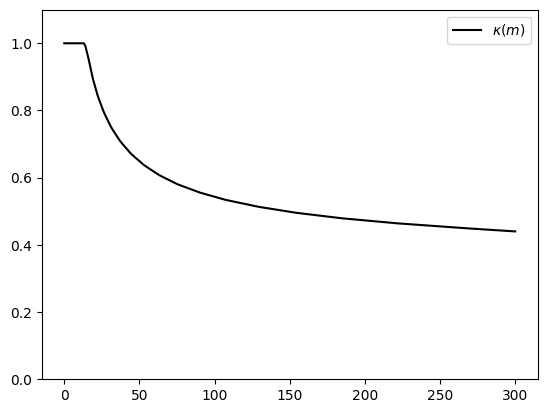
\includegraphics[width=0.6\textwidth]{kFunc_baseline.png}
    \caption{Optimal portfolio share with uncorrelated shocks}
    \label{fig:baseline_portfolio}
\end{figure}

It is obvious that this asymptotic value of $\k$ is increasing in the equity premium. Since the consumer is risk-averse, increasing the volatility of the returns to equity will decrease its attractiveness, thus reducing the optimal value of $\k$ upon an increase in $\s_{\nu}$. The only question, then, is the effect of a positive covariance between income shocks and asset returns on optimal asymptotic portfolio share.

\begin{figure}[h]
    \centering
    \begin{subfigure}{0.49\textwidth}
        \centering
        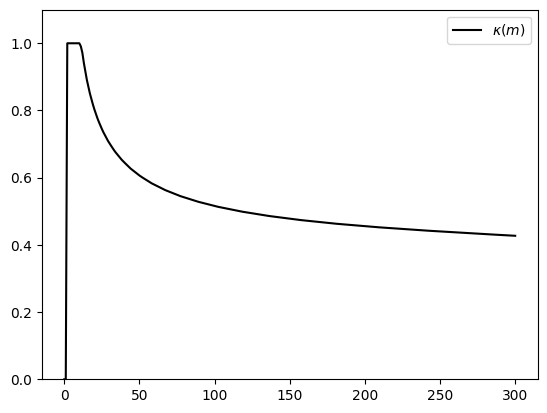
\includegraphics[width=0.8\textwidth]{kFunc_baseline_corrTransFull.png}
        \caption{Transitory shock ($\o_{\nu,\,\z} = 0.014$)}
        \label{subfig:correlated_baseline_transitory}
    \end{subfigure}
    \begin{subfigure}{0.49\textwidth}
        \centering
        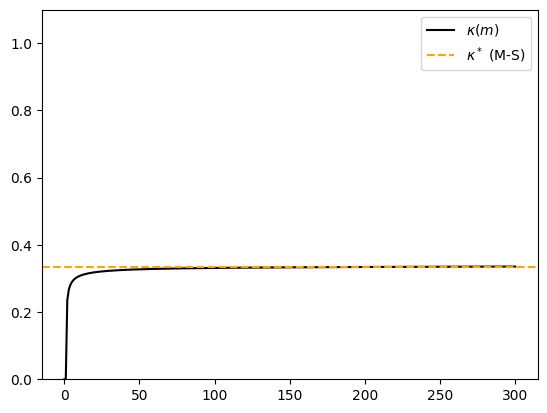
\includegraphics[width=0.8\textwidth]{kFunc_baseline_corr.png}
        \caption{Permanent shock ($\o_{\eta,\,\nu} = 0.008$)}
        \label{subfig:correlated_baseline_permanent}
    \end{subfigure}
    \caption{Optimal portfolio share with a positive correlation between income shocks and asset returns}
    \label{fig:correlated_shock_baseline}
\end{figure}

Figure \ref{fig:correlated_shock_baseline} shows how optimal portfolio share responds to a positive correlation between either of the income shocks and asset returns. Figure \ref{subfig:correlated_baseline_transitory} depicts the case when the transitory shock is correlated with asset returns. Since the optimal portfolio allocation is unaffected for all but the lowest values of $m$ (see section \ref{portfolio_low_wealth}), the asymptotic level of $\k$ remains the same as in the model with uncorrelated shocks. Figure \ref{subfig:correlated_baseline_permanent} shows the portfolio allocation rule under a moderate correlation between permanent income and asset return shocks. Even with a completely different optimal portfolio allocation rule, for high levels of wealth, the optimal portfolio share tends to similar values as in the case with no correlations.

The explanation for this behavior can be found by examining the optimal portfolio share condition, given by:
\[
\E_{t}\bs{(\Rfree_{t+1} - \Rfix)(\Gc_{t+1}c(m_{t+1}))^{-\rho}} = 0
\]
where
\[
m_{t+1} = \frac{\Rc_{t+1}}{\Gc_{t+1}}(m_{t} - c_{t}) + \z_{t+1}
\]
Unquestionably, the covariances between the shocks affect the realized values of $m_{t+1}$, and therefore the realizations of future consumption given by $c(m_{t+1})$. However, as $m_{t}$ becomes arbitrarily large, the ratio of labor income and present discounted value of human capital to assets tends to 0. As such, in the limit, irrespective of the covariances between the income shocks and asset returns, the consumer decides their portfolio share as if income is not a consideration. In other words, they behave like an individiual who has no labor income, and derives all income from the return on their investments \citep{Carroll2024}.

\begin{figure}[h]
    \centering
    \begin{subfigure}{0.49\textwidth}
        \centering
        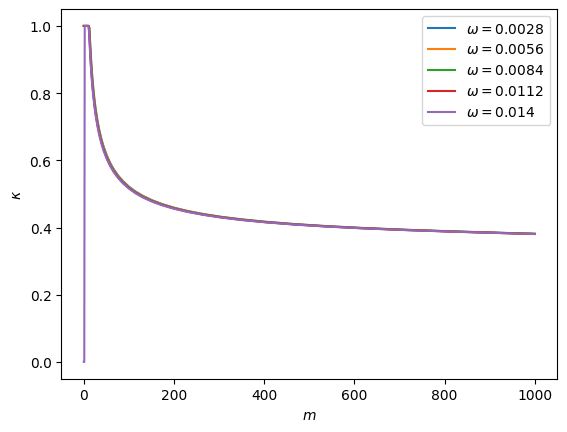
\includegraphics[width=0.8\textwidth]{ShareLimit_transInc_baseline.png}
        \caption{Transitory shock ($\o_{\nu,\,\z} = 0.014$)}
        \label{subfig:shareLimit_baseline_transitory}
    \end{subfigure}
    \begin{subfigure}{0.49\textwidth}
        \centering
        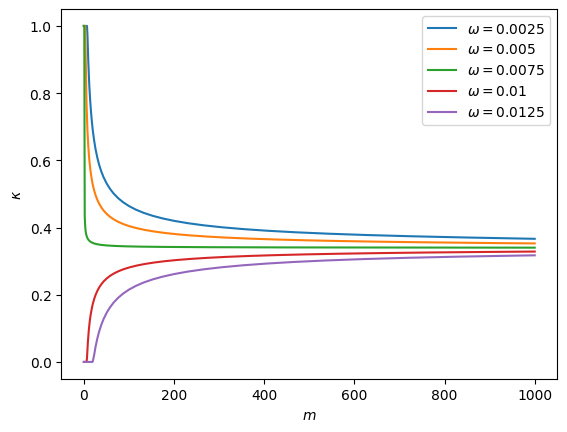
\includegraphics[width=0.8\textwidth]{ShareLimit_permInc_baseline.png}
        \caption{Permanent shock ($\o_{\eta,\,\nu} = 0.008$)}
        \label{subfig:shareLimit_baseline_permanent}
    \end{subfigure}
    \caption{Optimal portfolio share tends to the same value as $m\to \infty$}
    \label{fig:shareLimit_baseline}
\end{figure}

Figure \ref{fig:shareLimit_baseline} provides a rough idea of how the optimal portfolio rule behaves for different levels of correlation between income shocks and asset returns. Figure \ref{subfig:shareLimit_baseline_transitory} shows that correlations between transitory income shocks and asset returns hardly affect the portfolio allocation decision. However, while the portfolio allocation rule is indeed affected significantly by permanent income and asset return shock correlations, as seen in Figure \ref{subfig:shareLimit_baseline_permanent}, the share limit as $m \to \infty$ appears to be unaffected, as the portfolio allocation rules seem to converge. However, given the extremely large savings required to observe such convergence, which is unlikely to be observed of any agent in the model, a change in the correlation between the shocks would indeed affect the distribution of equity holdings. Section \ref{target_wealth} elaborates further on how the equity portfolio share at the target level of wealth is indeed extreme in this model.

\subsubsection{Optimal portfolio share at low wealth}\label{portfolio_low_wealth}

While optimal portfolio shares at large wealth levels are not affected much by the correlation between shocks, we can observe a stark change in the share of the risky asset among individuals whose wealths are less than twice of their permanent incomes.

\begin{figure}[h]
    \centering
    \begin{subfigure}{0.49\textwidth}
        \centering
        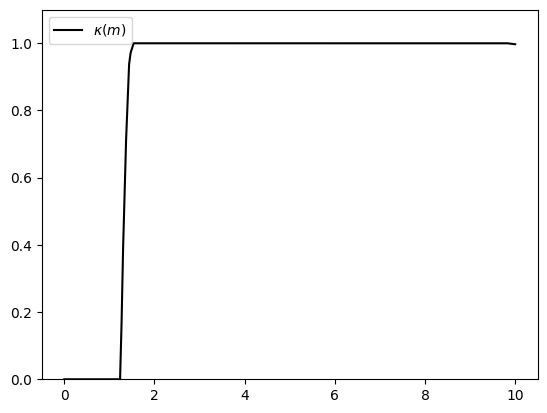
\includegraphics[width=0.8\textwidth]{kFunc_baseline_corrTrans.png}
        \caption{Transitory shock}
        \label{subfig:correlated_poor_transitory}        
    \end{subfigure}
    \begin{subfigure}{0.49\textwidth}
        \centering
        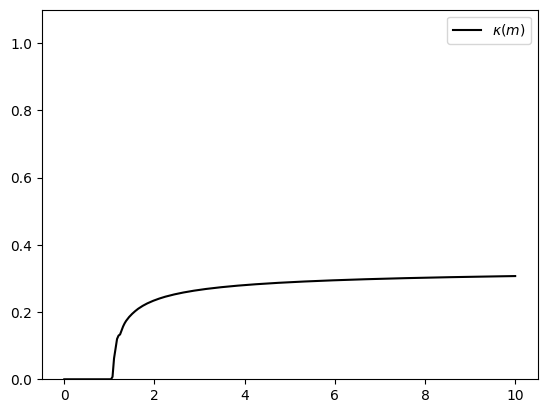
\includegraphics[width=0.8\textwidth]{kFunc_baseline_corrZoomed.png}
        \caption{Permanent shock}
        \label{subfig:correlated_poor_permanent}
    \end{subfigure}
    \caption{Individuals with low wealth invest all their savings in the risk-free asset}
    \label{fig:baseline_correlated_poor}
\end{figure}

Figure \ref{fig:baseline_correlated_poor} shows that agents with normalized wealth less than 2 (somewhere between 1 and 2 to be precise), invest all their savings in the risk-free asset, irrespective of whether asset returns are correlated with transitory or permanent income shocks. At low levels of savings, notice that $\z_{t+1}$ comprises the major component of $m_{t+1}$, and high covariance between $\nu_{t+1}$ and $\z_{t+1}$ implies that low values of $\z_{t+1}$ go with low values of $\nu_{t+1}$. Since the marginal utility of future consumption is high at low values of $m_{t+1}$, which coincides with low values of $\Rfree_{t+1}$, greater weight is placed on instances with low asset returns when taking the expectations in equation (\ref{eq:excess_return}). This lowers the optimal portfolio share of the risky asset, in this case to 0. The other situation is when $\nu$ is correlated with $\eta$. Given the equation of $m_{t+1}$, this actually reduces the variability in $c(m_{t+1})$. However, the positive correlation between $\nu$ and $\eta$ implies that when $\Rfree_{t+1} - \Rfix$ is negative, $\Gc_{t+1}$ is low, implying that $\Gc_{t+1}^{-\rho}$ is higher. Thus, the instances of negative return are weighted higher in the excess return equation. Supposing that $\nu$ and $\eta$ are perfectly correlated, if $\k  1$, then $m_{t+1} - \z_{t+1}$ becomes a constant, and the higher weight accorded to instances with negative return implies that the expectation becomes negative. On the other hand, if $\k = 0$, negative values of $\Rfree_{t+1} - \Rfix$ are coupled with low values of $\Gc_{t+1}$ and therefore higher $m_{t+1}$, implying that the lower marginal utility of normalized consumption under negative excess returns makes $\k = 0$ closer to optimality.

The second aspect is how the optimal portfolio share looks for slightly higher levels of wealth. Upto $m \approx 1.5$, agents consume almost all of their monetary resources and save next to nothing (see section \ref{consumption_baseline}). As such, the high MPC out of consumption causes variability in future monetary resources to translate into variability in future consumption at an almost one-to-one level. After a certain threshold, however, the MPC sharply falls, and the concavity of the consumption function ensures that it continues to fall. Moreover, due to the diminishing marginal utility of consumption and the very low magnitude of the marginal-marginal-utility of consumption, variability in $m_{t+1}$ translates to very little variability in $c(m_{t+1})^{-\rho}$. The analysis of the finite horizon model in section \ref{finite_horizon} highlights the particular relevance of the MPC channel on this effect.

In that light, see that the argument for why optimal $\k$ is low when permanent income shocks and returns are correlated does not crucially depend on the value of $a_{t+1}$ being extremely low, and the optimal $\k$ is always lower than the asymptotic value. However, when looking at the case with correlation between $\z$ and $\nu$, note that the only channel through which there is any effect is the marginal utility of consumption, or $c(m_{t+1})^{-\rho}$. By the discussion above, this has less of an effect at higher values of $m_{t+1}$, and the optimal portfolio allocation rule resembles the one in the model with uncorrelated shocks.

\subsubsection{Optimal consumption policy}\label{consumption_baseline}

While the properties of the consumption function in the buffer stock model are well understood, I reiterate some important features to augment that arguments provided above. Figure \ref{fig:baseline_consumption} shows the optimal consumption function.

\begin{figure}[h]
    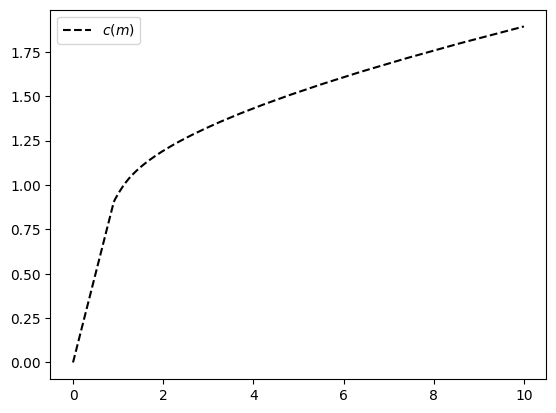
\includegraphics[width=0.6\textwidth]{cFunc_baseline_zoomed.png}
    \caption{Optimal consumption function in the buffer-stock model}
    \label{fig:baseline_consumption}
\end{figure}

Under the artificial no-borrowing constraint, the $c(m) \leq m$, which implies that $c$ is both defined only for $m \geq 0$ and has a kink at the point where the borrowing constraint begins to bind. For this region, the MPC is 1, implying that for low values of $m$, as remarked earlier, the total  savings rate is extremely low. However, the MPC sharply falls beyond this point. The code shows that the optimal consumption policy in the models with correlated shocks remains mostly unchanged. The low MPC for high values of $m$ thus leads to the ineffectiveness of transitory shocks in affecting optimal portfolio choice.

\subsection{Next-to-last period in finite-horizon}\label{finite_horizon}

Due to the convergence properties of the consumption function, we know that the optimal consumption rule in the finite-horizon model for periods sufficiently away from the last period closely approximate the infinite horizon consumption rule. As such, if the next period's consumption is similar to the infinite-horizon consumption, the optimal portfolio allocation rule should also be similar to the infinite-horizon rule. On the other end of this discussion is the period that is next to last.

The consumer in the last period knows that their optimization problem in the last period boils down to maximizing utility from current-period consumption, which implies that $c_T(m_T) = m_T$. The first useful feature of this is that it provides us with a consumption function for which we have an analytical expression, which allows us to rewrite the optimal portfolio allocation condition as:
\[
\E_{T-1}\bs{(\Rfree_{T} - \Rfix)(\Rc_{T}a_{T} + \Gc_{T}\z_{T})^{-\rho}}
\]
First, note that a permanent income growth and transitory income shock are identical in the last period, so to analyze one is to analyze the other. While the coincidence of negative values of $\Rfree_{T} - \Rfix$ and small values of $\Gc_{T}$ still holds true, the MPC out of total monetary resources is a constant 1. As a result, the only channel through which the portfolio choice problem differs at high $m_{T-1}$ as opposed to low is the marginal utility of consumption. Figure \ref{fig:last_prd_portfolio} shows that the optimal portfolio allocation is nearly identical to that in the infinite horizon problem, showing that the effect of correlations between permanent, as opposed to transitory, income shocks and asset returns for moderate values of $m_{T-1}$ is due to the low MPC out of transitory income. However, it also reiterates the point that the low MPC implied by the consumption function in the infinite-horizon problem plays a negligible role in affecting the portfolio choice of the extremely wealthy.

\subsection{Revisiting the excess return equation}

Appendix \ref{excess_return_approx} shows that the excess return equation that determines optimal portfolio allocation can be approximated by
\begin{equation}\label{eq:excess_return_linear}
    \E_{t}\bs{\Rfree_{t+1}} - \Rfix \approx \rho\text{cov}(\D \ln C_{t+1},\,\Rfree_{t+1})
\end{equation}
around steady state values of normalized consumption. Since real consumption change is approximately proportional to permanent income growth around the normalized steady state, a large increase in the covariance between permanent income growth shocks and shocks to $\Rfree_{t+1}$ would then imply that the excess return on equity is less than the covariance between consumption growth and the return on equity, scaled by the relative risk aversion coefficient. One thing to note here is that this approximation depends solely on the covariance, and not the correlation between permanent income growth and the risky rate of return. In fact, for fixed values of expected rates of return and volatility of the risky asset, one can observe that the optimal portfolio allocation rule does not depend much on the volatility of permanent income growth, just its covariance with the risky rate. For instance, under the baseline parameters for equity returns and various levels of permanent income growth volatility, one can observe that poor consumers make the switch from equity to the safe asset at approximately the same level of covariance between logged permanent income growth and equity return shocks.

A second aspect that can be analyzed about the optimal portfolio allocation rule is that for high enough covariance between permanent income growth and asset return shocks, the optimal portfolio share of equity is increasing in wealth, rather than decreasing as before. To understand this, we can look at the version of equation (\ref{eq:excess_return_linear}) that also takes into account the expected consumption growth,
\[
    \E_{t}\bs{\Rfree_{t+1}} - \Rfix \approx (1-\rho\E_{t}\bs{\D\ln C_{t+1}})^{-1}\rho\text{cov}(\D \ln C_{t+1},\,\Rfree_{t+1})
\]
At wealth levels lower than at which the normalized consumption steady state is attained, $\E_{t}\D\ln C_{t+1}$ is large,\footnote{Relative to the average level of permanent income growth} making equity a less desirable asset. On the other hand, for large values of $m_{t}$, as will be elborated on in the next section, agents engage in dissaving behavior (in normalized terms), implying that wealthy agents consume more out of wealth. In such a case, the covariance between consumption growth and equity returns become positive irrespective of the covariance between permanent income growth and equity returns. With $\D\ln C_{t+1}$ decreasing in wealth due to the previously mentioned dissaving behavior, the identical portfolio share limit across the parameterizations of the model can be explained by a convergence in the consumption growth rate as $m \to \infty$ and a decreasing component of permanent income growth in the covariance between consumption growth and equity returns.

\subsection{Behavior around target wealth}\label{target_wealth}

Till now, I have looked at the predictions of the model based on ad-hoc categorizations of poor and wealthy. However, the ability of the model to explain portfolio allocation decisions of individuals also depends on the saving behavior predicted by the model. \citet{Deaton1991} showed that under the satisfaction of a growth impatience condition, individuals save to achieve a target wealth, $m^*$. Assuming that a wealth distribution of agents facing idiosyncratic shocks would be centered around this target level, it would be informative to examine how agents behave at the target.
\begin{figure}[h]
    \centering
    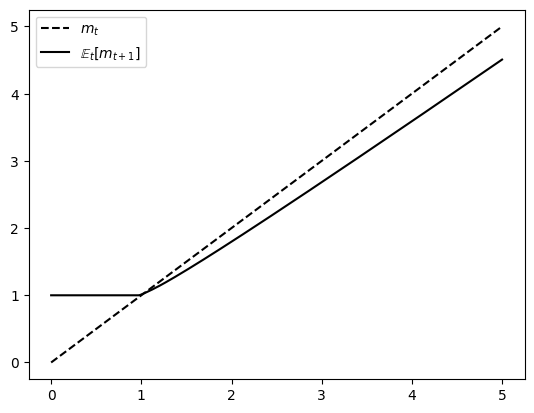
\includegraphics[width=0.6\textwidth]{wealth_transition_baseline.png}
    \caption{Expected next period normalized wealth conditional on current period wealth}
    \label{fig:wealth_transition}
\end{figure}
Figure \ref{fig:wealth_transition} shows how the dynamics of normalized wealth play out from period to period. For low values of $m_{t}$, where savings are zero, next-period wealth is entirely determined by the transitory income shock. Since the expected value of the shock is 1, future wealth is expected to be 1 for all low values of current wealth. Once the no-borrowing constraint stops binding, future wealth is increasing in current wealth. However, it is clear that expected future wealth is lower than current wealth for all values of current wealth slightly greater than 1. In fact, it can be numerically shown that the target level of saving is 2.8 percent of permanent income.

\begin{figure}[h]
    \centering
    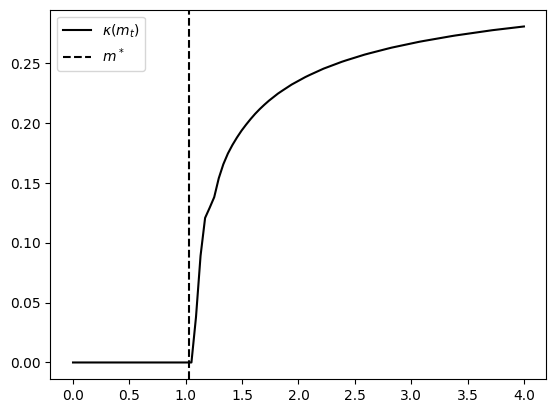
\includegraphics[width=0.6\textwidth]{kFunc_target_baseline.png}
    \caption{Optimal portfolio allocation at the target level of wealth}
    \label{fig:target_wealth_portfolio}
\end{figure}
Figure \ref{fig:target_wealth_portfolio} shows that at the target level of wealth, the optimal portfolio share accorded to equity is actually 0. This is because, under the no-borrowing constraint, the target level of wealth implies very little saving, or $a_{t+1} \approx 0$, where the optimal portfolio share was found to be $0$. If the consumer faces a negative shock to log transitory income, they still have some savings left to allow them to remain at the target level of wealth. When a consumer faces a positive shock to log transitory income, they begin participating in the stock market, and invest a small proportion of their savings in equity. However, from the target wealth, with all savings in the risk-free asset, a consumer's normalized wealth in the next period cannot exceed 1.4 under the current parameterization of the truncated distribution used to model log shocks to income. Then, a large proportion of agents in the wealth distribution should invest no more than 20 percent of their savings in equity, which, of course, would be an extreme prediction. It would, instead, be more intuitive if there was a smoother distribution over equity portfolio share.

A reason for these extreme findings is the binding no-borrowing constraint, and the consumer's heavy dependence on the transitory income for consumption. In fact, if the consumer experiences a negative shock to log transitory income, their consumption would drastically fall, as the target wealth lies just above the kink in the consumption function, and the MPC rises to 1 once the no-borrowing constraint binds. This means that the agent will begin saving once again only after they experience a positive transitory income shock, which prevents them from investing in equity at low levels of savings. In light of this, it can be observed that though the optimal portfolio share quickly rises to 1 in the case of a correlation between asset return and transitory income shocks, the target wealth actually lies below this region, implying that for levels of correlation high enough, the equity share at target wealth drops to 0.

In the next section, I modify the income process and relax the no-borrowing constraint to address this problem.